\documentclass[tikz,border=10pt]{standalone}
\usepackage{time}
\usetikzlibrary{shapes.geometric, shapes.multipart, arrows.meta, positioning, calc, fit, backgrounds, shadows, patterns}

% Define colors to match
\definecolor{blue}{RGB}{0,0,255}
\definecolor{orange}{RGB}{255,165,0}
\definecolor{dkgreen}{RGB}{0,100,0}
\definecolor{gray}{RGB}{128,128,128}
\definecolor{darkgray}{RGB}{64,64,64}

\begin{document}
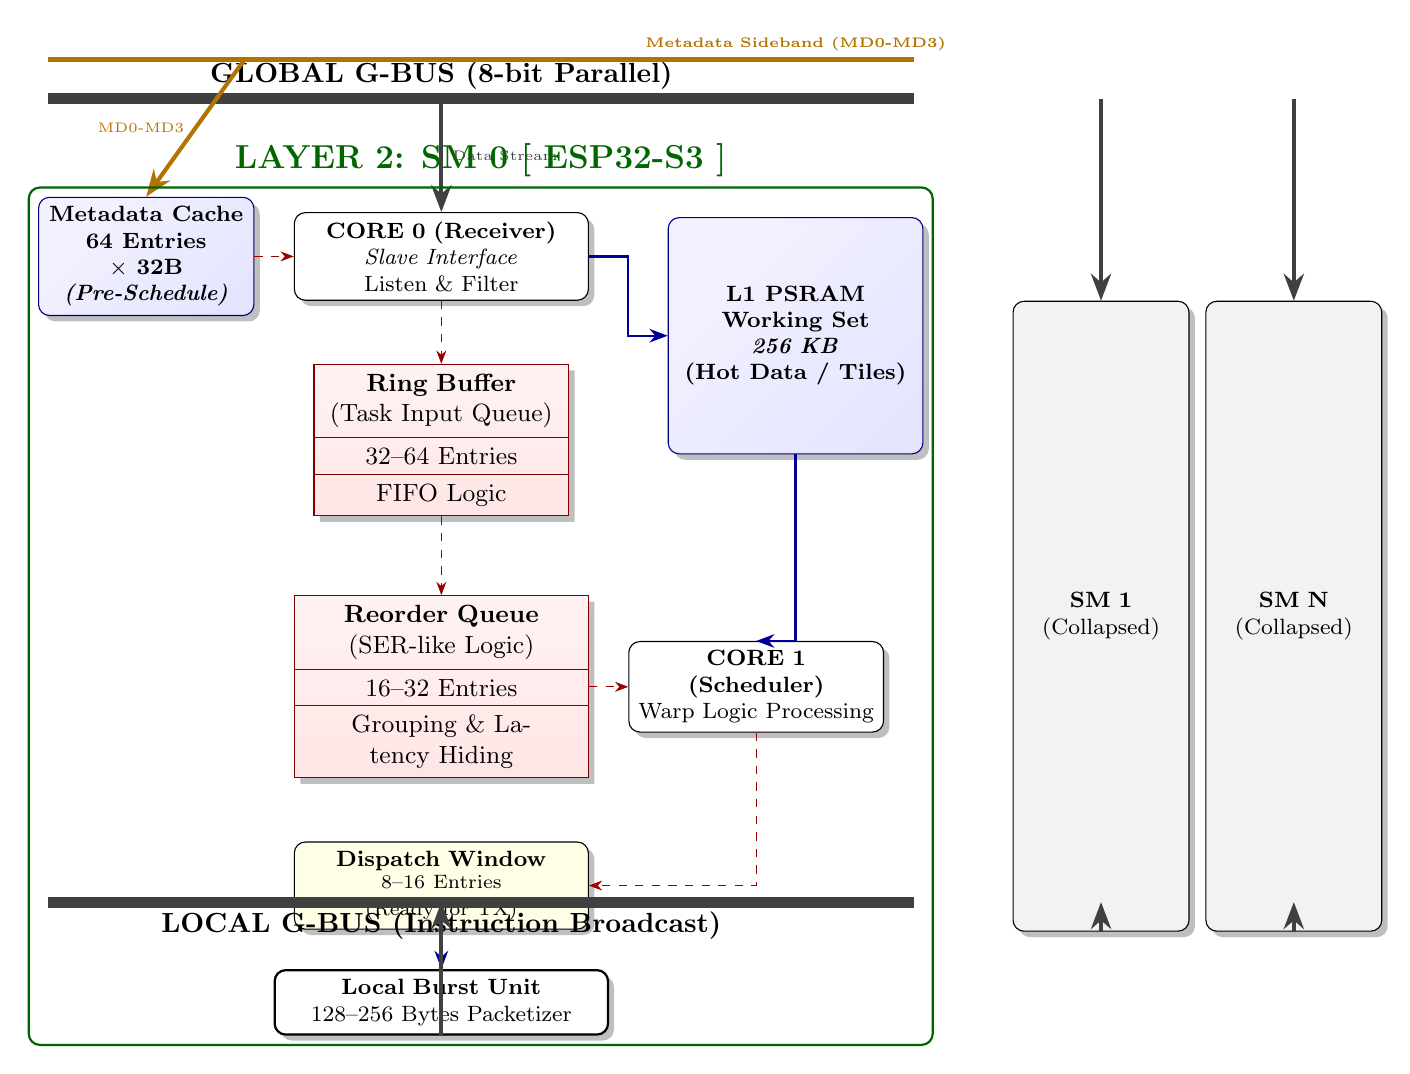
\begin{tikzpicture}[
    font=\sffamily,
    % 樣式定義
    component/.style={
        draw, fill=white, rounded corners, align=center, drop shadow, font=\footnotesize
    },
    core_block/.style={
        draw=gray, dashed, fill=gray!5, rounded corners, inner sep=10pt
    },
    memory_block/.style={
        draw=blue!50!black, top color=blue!5, bottom color=blue!10, 
        shading angle=45, rounded corners, align=center, drop shadow, font=\footnotesize\bfseries
    },
    queue_block/.style={
        draw=red!50!black, top color=red!5, bottom color=red!10, 
        rectangle split, rectangle split parts=3, align=center, drop shadow, font=\small
    },
    bus/.style={
        draw=darkgray, line width=4pt
    },
    bus_arrow/.style={
        ->, >=Stealth, thick, color=darkgray, line width=1.5pt
    },
    data_flow/.style={
        ->, >=Stealth, thick, blue!60!black
    },
    control_flow/.style={
        ->, >=Stealth, dashed, red!60!black
    }
]

    % --- 1. GLOBAL BUS (Top) ---
    \node (bus_label) at (0, 0) [above, font=\bfseries] {GLOBAL G-BUS (8-bit Parallel)};
    \draw[bus] (-5, 0) -- (6, 0);
    
    % Sideband visually separated - Moved upwards to avoid crossing
    \draw[bus, color=orange!70!black, line width=2pt] (-5, 0.5) -- (6, 0.5);
    \node at (4.5, 0.7) [font=\tiny\bfseries, text=orange!70!black] {Metadata Sideband (MD0-MD3)};

    % --- 2. ESP32-S3 SM 0 CONTAINER ---
    
    % --- CORE 0 AREA (Receiver) ---
    \node[component, text width=3.5cm] (rx_unit) at (0, -2) {
        \textbf{CORE 0 (Receiver)}\\
        \textit{Slave Interface}\\
        Listen \& Filter
    };

    % Metadata Cache (Sideband Processing)
    \node[memory_block, left=0.5cm of rx_unit, text width=2.5cm, fill=orange!10] (meta_cache) {
        \textbf{Metadata Cache}\\
        64 Entries $\times$ 32B\\
        \textit{(Pre-Schedule)}
    };

    % Connections from Bus - Adjusted path
    \draw[bus_arrow, orange!70!black] (-2.5, 0.5) -- node[left, font=\tiny] {MD0-MD3} (meta_cache.north);
    \draw[bus_arrow] (0, 0) -- node[right, font=\tiny] {Data Stream} (rx_unit.north);
    \draw[control_flow] (meta_cache) -- (rx_unit);

    % --- MEMORY & BUFFERS (Middle Layer) ---
    
    % L1 PSRAM (Big Shared Pool)
    \node[memory_block, right=1cm of rx_unit, text width=3cm, minimum height=3cm, anchor=north west, yshift=0.5cm] (psram) {
        \textbf{L1 PSRAM}\\
        \textbf{Working Set}\\
        \textit{256 KB}\\
        (Hot Data / Tiles)
    };

    % Ring Buffer (Task Queue)
    \node[queue_block, below=0.8cm of rx_unit, text width=3cm] (ring_buf) {
        \textbf{Ring Buffer}\\
        (Task Input Queue)
        \nodepart{second} 32--64 Entries
        \nodepart{third} FIFO Logic
    };

    % Data write flow
    \draw[data_flow] (rx_unit.east) -- ++(0.5,0) |- (psram.west);
    \draw[control_flow] (rx_unit.south) -- (ring_buf.north);

    % --- CORE 1 AREA (Scheduler) ---
    
    % Reorder Queue
    \node[queue_block, below=1cm of ring_buf, text width=3.5cm] (reorder_q) {
        \textbf{Reorder Queue}\\
        (SER-like Logic)
        \nodepart{second} 16--32 Entries
        \nodepart{third} Grouping \& Latency Hiding
    };

    % Core 1 Logic
    \node[component, right=0.5cm of reorder_q, text width=3cm] (core1_logic) {
        \textbf{CORE 1 (Scheduler)}\\
        Warp Logic Processing
    };

    % Dispatch Window - Moved text inside to avoid overlap
    \node[component, below=0.8cm of reorder_q, text width=3.5cm, fill=yellow!10] (dispatch) {
        \textbf{Dispatch Window}\\
        \scriptsize 8--16 Entries\\
        (Ready for TX)
    };

    % Burst Unit
    \node[component, below=0.5cm of dispatch, text width=4cm, draw=black, thick] (burst_unit) {
        \textbf{Local Burst Unit}\\
        128--256 Bytes Packetizer
    };

    % Core 1 Flows
    \draw[control_flow] (ring_buf.south) -- (reorder_q.north);
    \draw[data_flow] (psram.south) |- (core1_logic.north);
    \draw[control_flow] (reorder_q.east) -- (core1_logic.west);
    \draw[control_flow] (core1_logic.south) |- (dispatch.east);
    \draw[data_flow] (dispatch.south) -- (burst_unit.north);

    % --- FRAME FOR SM 0 ---
    \node[draw=green!40!black, thick, rounded corners, fit=(rx_unit) (meta_cache) (psram) (burst_unit), label={[green!40!black, font=\large\bfseries]north:LAYER 2: SM 0 [ ESP32-S3 ]}] (sm0_frame) {};

    % --- NEIGHBOR SMs (Collapsed) ---
    \node[component, right=1cm of sm0_frame, minimum height=8cm, text width=2cm, fill=gray!10] (sm1) {
        \textbf{SM 1}\\
        (Collapsed)
    };
    \node[component, right=0.2cm of sm1, minimum height=8cm, text width=2cm, fill=gray!10] (smn) {
        \textbf{SM N}\\
        (Collapsed)
    };
    
    % Bus connections for neighbors - Aligned vertically
    \draw[bus_arrow] (sm1.north |- 0,0) -- (sm1.north);
    \draw[bus_arrow] (smn.north |- 0,0) -- (smn.north);

    % --- 3. LOCAL BUS (Bottom) ---
    % Increased spacing to avoid overlap
    \coordinate (local_bus_y) at ($(burst_unit.south) + (0,-1.2)$);
    \draw[bus] (-5, -10.2) -- (6, -10.2);
    
    % Moved label to avoid overlapping with line
    \node at (0, -10.5) [font=\bfseries] {LOCAL G-BUS (Instruction Broadcast)};

    % Output connection - Extended length
    \draw[bus_arrow] (burst_unit.south) -- (0, -10.2);
    \draw[bus_arrow] (sm1.south) -- (sm1.south |- 0, -10.2);
    \draw[bus_arrow] (smn.south) -- (smn.south |- 0, -10.2);

\end{tikzpicture}
\end{document}
